\subsection{Parallelism}

\placelogofalse
\begin{frame}{Non-uniform Memory Access (NUMA)}
\begin{columns}
\column{0.48\linewidth}
\centering
\begin{outline}
  \1 Distribute index partitions across NUMA nodes
  \1 Affinity based scheduling and work-stealing
  \1 Experimental Results:
  \2 Exhibits linear scalability
  \2 Maximizes memory bandwidth utilization
  \2 4x speedup over non-NUMA aware
\end{outline}

\column{0.48\linewidth}
\begin{center}
\centering
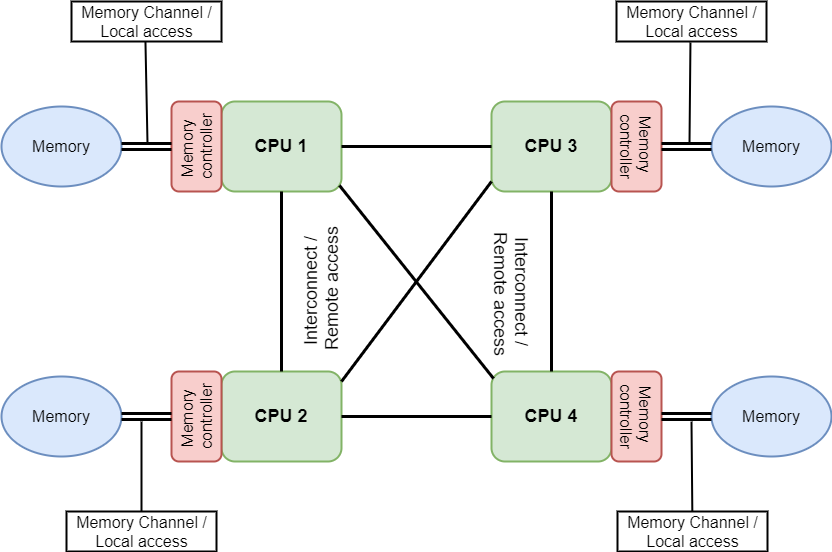
\includegraphics[width=4.0cm]{assets/NUMA.png}

{\tiny From \href{https://docs.lxp.lu/system/images/NUMA.png}{MeluXina}}

\vspace{0.5cm}

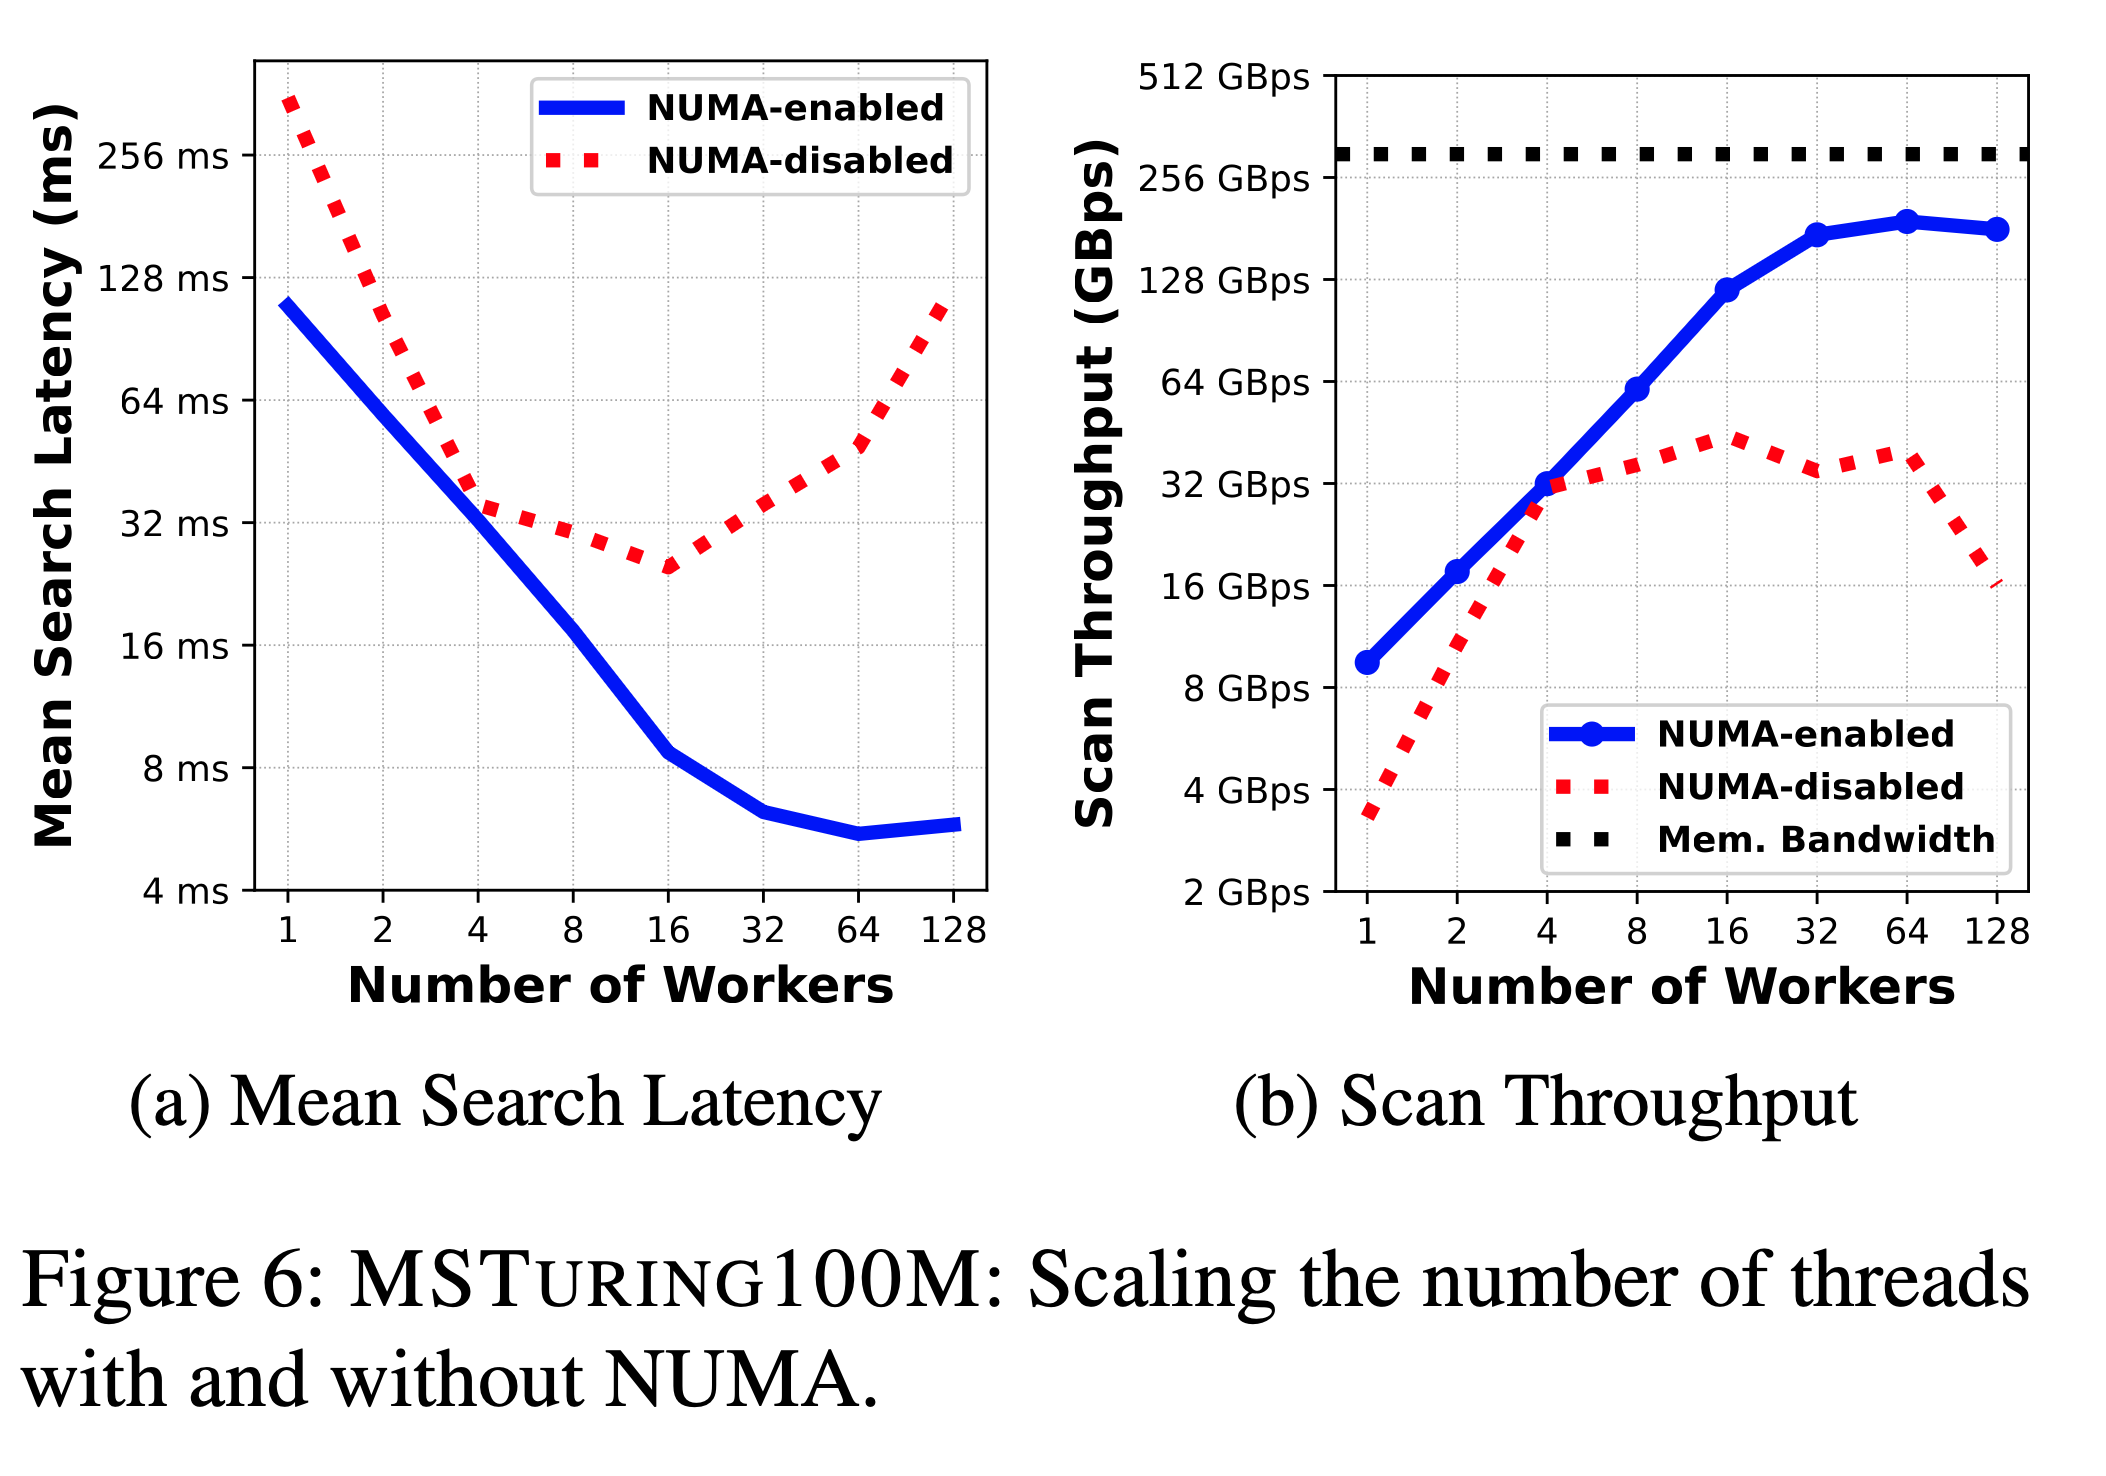
\includegraphics[width=5.5cm]{assets/numa_fig.png}
\end{center}
\end{columns}
\end{frame}
\placelogotrue
